\begin{subfigure}[h]{0.50\textwidth}
        \centering
        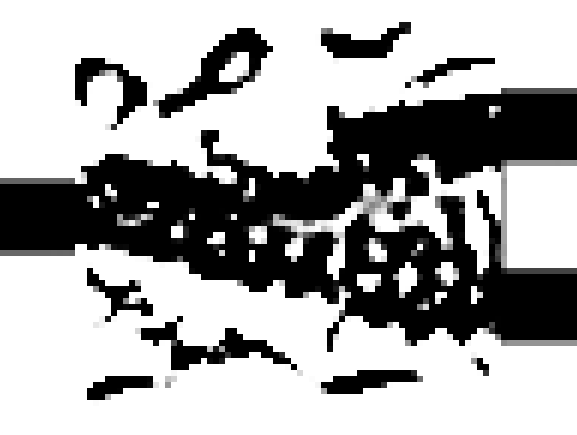
\includegraphics[width=0.8\textwidth]
        {fig/sim/simyjunction40.png}
        \caption{Simulated Y-junction structure with smallest feature size 40 nm.}
    \end{subfigure}%
    ~ 
    \begin{subfigure}[h]{0.50\textwidth}
        \centering
        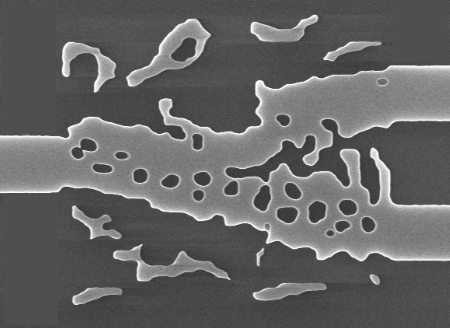
\includegraphics[width=0.8\textwidth]
        {fig/SEM/SEMyjunction40zoom.png}
        \caption{Fabricated Y-junction structure with smallest feature size 40 nm.}
    \end{subfigure}
    
    \vspace{5 mm}
    
    \begin{subfigure}[h]{0.50\textwidth}
        \centering
        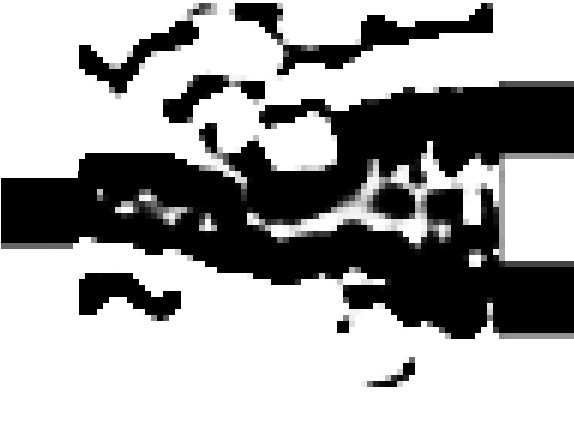
\includegraphics[width=0.8\textwidth]
        {fig/sim/simyjunction60.png}
        \caption{Simulated Y-junction structure with smallest feature size 60 nm.}
    \end{subfigure}%
    ~ 
    \begin{subfigure}[h]{0.50\textwidth}
        \centering
        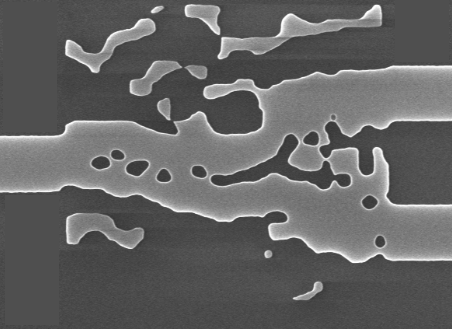
\includegraphics[width=0.8\textwidth]
        {fig/SEM/SEMyjunction60zoom.png}
        \caption{Fabricated Y-junction structure with smallest feature size 60 nm.}
    \end{subfigure}
    
    \vspace{5 mm}
    
    \begin{subfigure}[h]{0.50\textwidth}
        \centering
        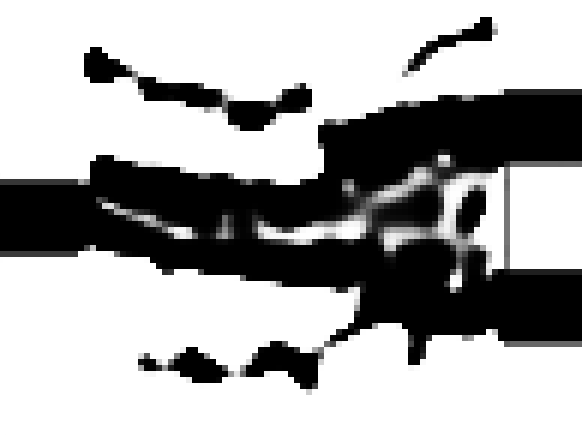
\includegraphics[width=0.8\textwidth]
        {fig/sim/simyjunction80.png}
        \caption{Simulated Y-junction structure with smallest feature size 80 nm.}
    \end{subfigure}%
    ~ 
    \begin{subfigure}[h]{0.50\textwidth}
        \centering
        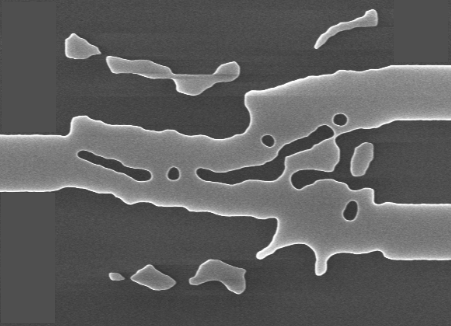
\includegraphics[width=0.8\textwidth]
        {fig/SEM/SEMyjunction80zoom.png}
        \caption{Fabricated Y-junction structure with smallest feature size 80 nm.}
    \end{subfigure}